% !TeX program = lualatex
\documentclass[a4paper,11pt]{article}
\usepackage{luatexja}
\usepackage[haranoaji]{luatexja-preset}
\usepackage{amsmath,amssymb,bm}
\usepackage[margin=24mm]{geometry}
\usepackage{tikz}
\usepackage{titlesec}
\titleformat{\section}{\large\bfseries}{\thesection}{1em}{}
\titlespacing*{\section}{0pt}{14pt}{5pt}
\setlength{\parindent}{1em}
\setlength{\parskip}{4pt}
\renewcommand{\baselinestretch}{1.18}
\newcommand{\Q}[2]{\section*{Q#1\quad #2}}
\newcommand{\conj}[1]{\overline{#1}}
\DeclareMathOperator{\atanTwo}{atan2}
\begin{document}
\begin{center}
{\LARGE\bfseries フーリエ変換について：設問解答}\\[6pt]
{原本：0064\_260928073535\_001.pdf}
\end{center}
\noindent\textbf{対象範囲：}原本にある設問はQ1〜Q14である。(15)〜(17)は式番号であり、Q15〜Q17という設問は原本にない。本書では全14問に解答する。式番号への言及は原本の番号を指す。

\noindent\textbf{規約：}$\omega_0=2\pi/T$、$T>0$、$i^2=-1$ とする。原本どおり $\cos$ の係数を $b_n$、$\sin$ の係数を $a_n$ とする。実数信号を基本とし、複素数信号との違いは必要な箇所に明記する。

\Q{1}{基本振動と5倍振動}
原本(1)の $n=1$ と $n=5$ の項をそれぞれ取り出せばよい。
\[
\boxed{f_1(t)=b_1\cos(\omega_0t)+a_1\sin(\omega_0t)}
\]
\[
\boxed{f_5(t)=b_5\cos(5\omega_0t)+a_5\sin(5\omega_0t)}
\]
角周波数はそれぞれ $\omega_0$、$5\omega_0$、周期は $T$、$T/5$ である（係数がともに0なら、その振動成分は存在しない）。

\Q{2}{振動項の時間平均と定数項}
時間平均を1周期（またはその整数倍）での平均とする。$n\geq1$ に対し、任意の $\tau$ について
\[
\frac1T\int_\tau^{\tau+T}\cos(n\omega_0t)\,dt
=\frac1T\int_\tau^{\tau+T}\sin(n\omega_0t)\,dt=0.
\]
したがって各振動項の平均は0であり、
\[
\boxed{\langle f\rangle=\frac1T\int_\tau^{\tau+T}f(t)\,dt=\frac{b_0}{2}}
\]
である。$b_0/2$ は信号の平均値、すなわち直流成分を表す。任意の長さの有限時間区間では、振動項の平均は必ずしも0にならない。

\Q{3}{振幅と位相のずれ}
$\theta=n\omega_0t$ とおく。$A_n>0$ のとき
\[
\boxed{A_n=\sqrt{a_n^2+b_n^2}},\qquad
\phi_n=\atanTwo(a_n,b_n),
\]
\[
b_n\cos\theta+a_n\sin\theta=A_n\cos(\theta-\phi_n).
\]
ここで $\atanTwo(y,x)$ は $\cos\phi=x/\sqrt{x^2+y^2}$、$\sin\phi=y/\sqrt{x^2+y^2}$ を満たす象限込みの偏角である。
$\cos(\theta+\delta_n)$ の形での位相差は
\[
\boxed{\delta_n=-\phi_n=\atanTwo(-a_n,b_n)\pmod{2\pi}}.
\]
$\phi_n$ は $\cos(\theta-\phi_n)$ の形での遅れを表す。$A_n=0$ の場合、位相は定義されない。
\newpage
\Q{4}{複素フーリエ係数}
Eulerの公式から
\[
\cos\theta=\frac{e^{i\theta}+e^{-i\theta}}2,\qquad
\sin\theta=\frac{e^{i\theta}-e^{-i\theta}}{2i}.
\]
よって、$n>0$ に対して
\[
b_n\cos(n\omega_0t)+a_n\sin(n\omega_0t)
=\frac{b_n-ia_n}{2}e^{in\omega_0t}
+\frac{b_n+ia_n}{2}e^{-in\omega_0t}.
\]
原本(3)との比較により
\[
\boxed{c_0=\frac{b_0}{2},\quad c_n=\frac{b_n-ia_n}{2},\quad
c_{-n}=\frac{b_n+ia_n}{2}\quad(n>0)}.
\]
逆の関係は $b_n=c_n+c_{-n}$、$a_n=i(c_n-c_{-n})$ である。

\Q{5}{複素表示での3倍振動}
実際の3倍振動を表すには正負両方の周波数を組にする。
\[
\boxed{f_3(t)=c_3e^{i3\omega_0t}+c_{-3}e^{-i3\omega_0t}}
=b_3\cos(3\omega_0t)+a_3\sin(3\omega_0t).
\]
$c_3e^{i3\omega_0t}$ だけでは正周波数側の項のみであり、一般には実数の振動にならない。

\Q{6}{実数信号の共役対称性}
$a_n,b_n$ が実数なのでQ4より
\[
\boxed{c_{-n}=\conj{c_n}}.
\]
また、積分表示を用いても、$f(t)$ が実数であることから
\[
\conj{c_n}
=\frac1T\int_\tau^{\tau+T}f(t)e^{in\omega_0t}\,dt=c_{-n}
\]
となる。特に $c_0$ は実数である。

\Q{7}{複素係数の絶対値と偏角}
$c_n=|c_n|e^{i\delta_n}$ と共役対称性を使うと
\begin{align*}
f_n(t)&=c_ne^{in\omega_0t}+\conj{c_n}e^{-in\omega_0t}\\
&=2|c_n|\cos(n\omega_0t+\delta_n).
\end{align*}
したがって
\[
\boxed{|c_n|=\frac{A_n}{2}=\frac{\sqrt{a_n^2+b_n^2}}{2}},\qquad
\boxed{\delta_n=\arg c_n=\atanTwo(-a_n,b_n)\pmod{2\pi}}.
\]
絶対値 $|c_n|$ は実際の余弦振動の振幅の半分、偏角は余弦を基準とした位相差である。振幅が半分になるのは、1つの実振動を正負2つの周波数成分に分けているためである。$c_n=0$ では偏角は定義されない。
\newpage
\Q{8}{指数関数の直交関係}
$p=n-m\in\mathbb Z$ とおく。$p=0$ なら被積分関数は1なので積分値は $T$。$p\ne0$ なら
\begin{align*}
\int_\tau^{\tau+T}e^{ip\omega_0t}\,dt
&=\frac{e^{ip\omega_0\tau}(e^{ip\omega_0T}-1)}{ip\omega_0}\\
&=\frac{e^{ip\omega_0\tau}(e^{i2\pi p}-1)}{ip\omega_0}=0.
\end{align*}
したがって、任意の $\tau$ に対して原本(4)が成り立つ。
\[
\boxed{\int_\tau^{\tau+T}e^{i(n-m)\omega_0t}\,dt=T\delta_{nm}}
\]
ここで $\delta_{nm}$ は $n=m$ のとき1、それ以外で0のKroneckerのデルタである。

\Q{9}{係数の積分公式}
原本(3)に $e^{-im\omega_0t}$ をかけて1周期積分すると、Q8より
\begin{align*}
\int_\tau^{\tau+T}f(t)e^{-im\omega_0t}\,dt
&=\sum_{n=-\infty}^{\infty}c_n
\int_\tau^{\tau+T}e^{i(n-m)\omega_0t}\,dt\\
&=\sum_{n=-\infty}^{\infty}c_nT\delta_{nm}=Tc_m.
\end{align*}
ゆえに
\[
\boxed{c_m=\frac1T\int_\tau^{\tau+T}f(t)e^{-im\omega_0t}\,dt}.
\]
上の計算は、例えばフーリエ部分和が $f$ に $L^2$ 収束する場合に正当化できる。まず有限和について積分し、その後、内積の連続性により極限を取ればよい。有限区間の通常の区分的連続関数は $L^2$ に属するため、この意味で扱える。各点での級数の収束は別の問題である。

\Q{10}{フーリエ成分の意味}
フーリエ成分 $X(\omega)$ は，信号 $f(t)$ の中に，\textbf{角周波数 $\omega$ の波がどのくらい含まれているか，また，その波の位相がどのようにずれているか}を表す複素数である。角周波数は振動の速さを表し，周波数（Hz）の $2\pi$ 倍である。

例えば，音の波形には低い音や高い音の振動が重なっている。フーリエ変換をすると，その波形を周波数ごとに調べて，どの高さの音の成分が強いかを知ることができる。

式(10)にEulerの公式 $e^{-i\omega t}=\cos(\omega t)-i\sin(\omega t)$ を使うと，
\[
X(\omega)
=\int_{-\infty}^{\infty}f(t)\cos(\omega t)\,dt
-i\int_{-\infty}^{\infty}f(t)\sin(\omega t)\,dt
\]
となる。つまり，$f(t)$ と，調べたい角周波数の $\cos$，$\sin$ をそれぞれ掛けて積分している。この計算によって，その角周波数の波の成分を調べられる。

$X(\omega)$ を極形式で
\[
X(\omega)=|X(\omega)|e^{i\phi(\omega)}
\]
と書くと，次のように意味づけられる。
\begin{itemize}
\item 絶対値 $|X(\omega)|$：その角周波数の成分の大きさを表す。
\item 偏角 $\phi(\omega)$：$\cos(\omega t)$ を基準とした位相のずれを表す。
\end{itemize}
位相のずれとは，波の山や谷が現れるタイミングのずれのことである。ただし，$X(\omega)=0$ のときには，その成分の位相は決められない。

なお，フーリエ変換では周波数が連続しているため，$|X(\omega)|$ をそのまま1本の波の振幅と考えるわけではない。式(12)のように，$X(\omega)$ に $e^{i\omega t}$ を掛け，全角周波数について積分し，$2\pi$ で割ることで，元の信号 $f(t)$ が得られる。
\newpage
\Q{11}{DFTの周波数添字の周期性}
原本(16)の規約は
\[
X_l=\Delta t\sum_{k=0}^{N-1}x_ke^{-i2\pi lk/N},\qquad \Delta t>0.
\]
$k$ が整数であるため $e^{-i2\pi k}=1$ であり、
\begin{align*}
X_{l+N}&=\Delta t\sum_{k=0}^{N-1}x_ke^{-i2\pi(l+N)k/N}\\
&=\Delta t\sum_{k=0}^{N-1}x_ke^{-i2\pi lk/N}e^{-i2\pi k}=X_l.
\end{align*}
従って $\boxed{X_{l+N}=X_l}$。この性質は複素数データについても成立する。

\Q{12}{離散標本では異なる周波数を区別できない理由}
標本時刻を $t_k=k\Delta t$、標本化角周波数を $\omega_s=2\pi/\Delta t$ とすると
\[
e^{i(\omega+l'\omega_s)t_k}
=e^{i\omega t_k}e^{i2\pi l'k}=e^{i\omega t_k}\qquad(l'\in\mathbb Z).
\]
連続時間では異なる波でも、周波数差が標本化角周波数の整数倍なら全標本点の値が同じになる。この現象を\textbf{エイリアシング（折り返し）}という。

下図では、横軸を $u=t/\Delta t$ とし、
\[
g_1(u)=\cos(2\pi u/8),\qquad g_2(u)=\cos(2\pi\cdot9u/8)
\]
を比較する。これは $N=8$、$l=1$ と $l+N=9$ の例である。整数 $u=k$ にある黒点では両曲線が一致する。DFTに使う8点は $k=0,\ldots,7$ であり、$k=8$ は次周期の先頭を参考として表示した。
\begin{center}
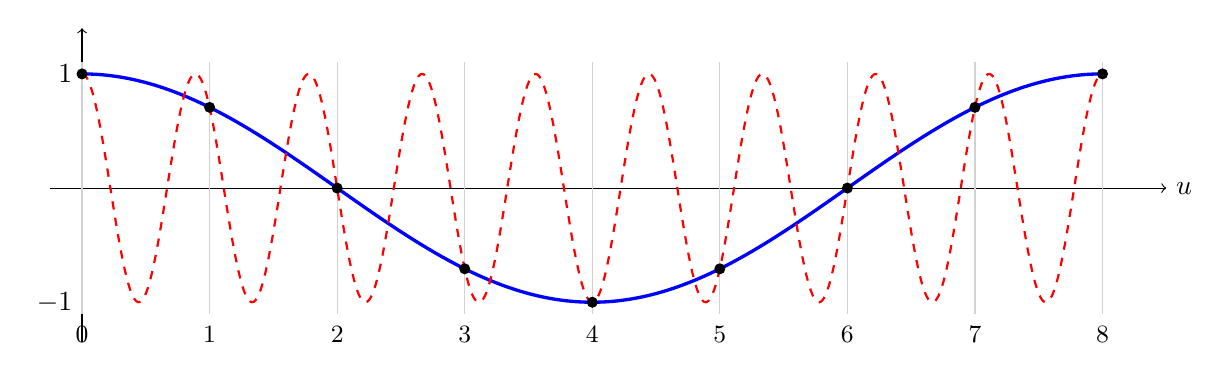
\begin{tikzpicture}[x=1.62cm,y=1.45cm]
\draw[->] (-.25,0)--(8.5,0) node[right] {$u$};
\draw[->] (0,-1.35)--(0,1.4);
\foreach \k in {0,...,8} {
 \draw[gray!35] (\k,-1.1)--(\k,1.1);
 \node[below] at (\k,-1.13) {\small $\k$};
}
\node[left] at (0,1) {$1$};\node[left] at (0,-1) {$-1$};
\draw[blue,very thick,domain=0:8,samples=201] plot (\x,{cos(45*\x)});
\draw[red,dashed,thick,domain=0:8,samples=601] plot (\x,{cos(405*\x)});
\foreach \k in {0,...,8} \fill (\k,{cos(45*\k)}) circle (2pt);
\end{tikzpicture}

{\small 青実線：$g_1$（低周波）、赤破線：$g_2$（高周波）、黒点：共通の標本値。}
\end{center}
DFTの周波数刻みは $\Delta\omega=2\pi/(N\Delta t)$ なので
\[
(l+N)\Delta\omega-l\Delta\omega=N\Delta\omega=\omega_s.
\]
これがQ11の添字の周期性に対応する。標本値だけから区別できないのは連続時間信号の周波数であり、有限個の標本値自体はQ14の逆DFTで復元できる。連続時間信号を一意に復元するには帯域制限などの追加条件が必要である。
\newpage
\Q{13}{$X_{N-2}$ と $X_2$ の関係}
原本のように $x_k$ が実数なら、
\begin{align*}
X_{N-2}
&=\Delta t\sum_{k=0}^{N-1}x_ke^{-i2\pi(N-2)k/N}\\
&=\Delta t\sum_{k=0}^{N-1}x_ke^{i4\pi k/N}
=\conj{X_2}.
\end{align*}
従って
\[
\boxed{X_{N-2}=\conj{X_2}},\qquad
|X_{N-2}|=|X_2|.
\]
非零であれば偏角は互いに符号が逆である（$2\pi$ を法として）。一般には実部が等しく虚部が逆符号なので、$X_{N-2}=X_2$ とは限らない。複素数データにはこの共役関係は一般に成り立たない。

一般形は $X_{(-l)\bmod N}=\conj{X_l}$ である。$X_0$ と、$N$ が偶数の場合の $X_{N/2}$ は実数となる。特に $N=4$ なら $N-2=2$ であり、$X_2$ 自体が実数である。

\Q{14}{逆DFTの導出}
原本の順変換には $\Delta t$ が付いているため、逆変換は
\[
\boxed{x_j=\frac1{N\Delta t}\sum_{l=0}^{N-1}X_l
 e^{i2\pi lj/N}\qquad(j=0,1,\ldots,N-1)}.
\]
$W_N=e^{-i2\pi/N}$ を用いれば
\[
\boxed{x_j=\frac1{N\Delta t}\sum_{l=0}^{N-1}X_l(W_N)^{-jl}}.
\]
\textbf{導出：}有限和の直交関係
\[
\sum_{l=0}^{N-1}e^{i2\pi l(j-k)/N}
=\begin{cases}N&j=k,\\0&j\ne k\end{cases}
\qquad(0\leq j,k<N)
\]
を用いる。$j\ne k$ の場合は、公比 $r=e^{i2\pi(j-k)/N}\ne1$、$r^N=1$ なので、等比級数の和 $(1-r^N)/(1-r)$ が0になる。
順変換を代入すると
\begin{align*}
\frac1{N\Delta t}\sum_{l=0}^{N-1}X_le^{i2\pi lj/N}
&=\frac1N\sum_{k=0}^{N-1}x_k
\sum_{l=0}^{N-1}e^{i2\pi l(j-k)/N}\\
&=\frac1N\sum_{k=0}^{N-1}x_kN\delta_{jk}=x_j.
\end{align*}
これは有限次元の恒等式であり、複素数データにも成立する。
また $\Delta\omega=2\pi/(N\Delta t)$ より、前置係数は
\[
\frac1{N\Delta t}=\frac{\Delta\omega}{2\pi}
\]
とも書け、連続逆変換の規約と対応する。順変換に $\Delta t$ を付けない別規約での逆変換係数 $1/N$ と混同しないこと。

\vfill
\noindent{\small\textbf{レビューについて：}本解答は別のAIエージェントによる独立した数学レビューと数値検算を実施して作成した。実在の専門家による査読・承認を示すものではない。詳細は同梱のレビュー記録を参照。}
\end{document}
